For mobile and robotics applications a real-time encoder is needed. Hardware based real-time video encoders are expensive and not massively produced, thus their availability is limited. Creating one with off-the-shelf components opens the potential users. Two different models chosen whose computational cost was low enough to keep them operating at real-time and had kept biological plausibility constraints.


\subsection{General purpose computing in the graphics processor unit}

GPU History
GPU programming 
OpenCL
Memory hierarchy

\subsection{The foveal pit model}

The highest resolution area of the eye is the foveal pit (see section \ref{sec:vision:eye}). A functional model for this region of the retina was developed by \citeauthor{basab-model}, they called the implementation the \emph{Filter-overlap Correction algorithm} (FoCal)\cite{basab-model}. It's based on the response and physiology of the fovea. The authors concluded that using four different layers of ganglion cells, most of the visually relevant information could be recovered after encoding. Furthermore, the encoder outputs a collection of rank-ordered spike trains. 

The ganglion cells themselves where modelled using Difference of Gaussians (DoG), Equation \ref{eq-dog}. 

\begin{equation}
\label{eq-dog}
DoG_w(x,y) = \pm\frac{1}{2\pi\sigma_{w,c}^2}e^{\frac{-(x^2 + y^2)}{2\sigma_{w,c}^2}}
\mp\frac{1}{2\pi\sigma_{w,s}^2}e^{\frac{-(x^2 + y^2)}{2\sigma_{w,s}^2}}
\end{equation}

The size of the receptive field of the simulated cells depends on the layer they belong to, this is reflected in the convolution kernel's width and parameters. Variables $\sigma_{w,c}$ and $\sigma_{w,s}$ are the standard deviation for the centre and surround components of the DoGs for layer $w$.  The signs for the equation will be ($-$,$+$) if the ganglion cell is \emph{off-centre} and ($+$,$-$) if it is \emph{on-centre}. The parameters for this equation can be found in table \ref{tab-kernel-specs}.

\begin{table}[htb]
  \caption{Simulation parameters for ganglion cells}
  \centering
  \bgroup
  \def\arraystretch{1.4}
  
  %  \begin{TAB}(r,1em,1.5em){|c|c|c|c|c|}{|c|c|c|c|c|} 
  \begin{tabular}{c c c c c c}
    \begin{minipage}{1cm}Layer \end{minipage}& 
    \begin{minipage}{2cm}Behaviour \end{minipage}&
    \begin{minipage}{1cm} \centering Matrix width \end{minipage}&  
    \begin{minipage}{2.5cm}\centering Centre \\std. dev. ($\sigma_c$)\end{minipage} & 
    \begin{minipage}{2.5cm}\centering Surround \\std. dev. ($\sigma_s$)\end{minipage} & 
    \begin{minipage}{2.5cm}\centering Sampling resolution \\(cols, rows)\end{minipage} \\
    \hline
    \begin{minipage}{1cm}\vspace*{0.1cm} \centering1 \end{minipage} &
    \begin{minipage}{2cm}\textsc{off}-centre \vspace*{0.005cm} \end{minipage}& 
    \begin{minipage}{0.5cm}\centering$3$ \end{minipage}& 
    $0.8$ & $6.7 \times \sigma_c$ & 1, 1\\
    \begin{minipage}{1cm}\centering 2 \end{minipage} & 
    \begin{minipage}{2cm}\textsc{on}-centre \vspace*{0.005cm}\end{minipage} & 
    \begin{minipage}{0.5cm}\centering $11$ \end{minipage}& 
    $1.04$ & $6.7 \times \sigma_c$ &  1, 1\\
    \begin{minipage}{1cm}\centering 3 \end{minipage} &
    \begin{minipage}{2cm}\textsc{off}-centre \vspace*{0.005cm}\end{minipage} & 
    \begin{minipage}{1cm}\centering $61$ \end{minipage}& 
    $8$ & $4.8 \times \sigma_c$ & 5, 3 \\
    \begin{minipage}{1cm}\centering 4 \end{minipage} & 
    \begin{minipage}{2cm}\textsc{on}-centre \vspace*{0.005cm}\end{minipage} & 
    \begin{minipage}{0.5cm}\centering $243$\end{minipage} &
    $10.4$ & $4.8 \times \sigma_c$ & 5, 3
  \end{tabular}
  \label{tab-kernel-specs}
  \egroup
  \vspace*{-5pt}
\end{table}

For each cell type, a convolution kernel must be computed and stored in a matrix ($DoG_{w}$). For each element in the matrix we use Equation \ref{eq-dog}, substituting parameters specified in Table \ref{tab-kernel-specs} and integer valued $x$-$y$ coordinates whose origin is the centre of the matrix. For example, for the $3\times3$ kernel (layer 1 cells), the upper-left value would be calculated as follows:

\begin{align}
\label{eq-dog-3x3}
DoG_3(x,y) &= -\frac{1}{2\pi\sigma_{3,c}^2}e^{\frac{-(x^2 + y^2)}{2\sigma_{3,c}^2}}
+ \frac{1}{2\pi\sigma_{3,s}^2}e^{\frac{-(x^2 + y^2)}{2\sigma_{3,s}^2}} \\
DoG_3(-1,-1) &= -\frac{1}{2\cdot\pi\cdot 0.8^2}e^{\frac{-((-1)^2 + (-1)^2)}{2\cdot 0.8^2}}
+ \frac{1}{2\cdot\pi\cdot 5.36^2}e^{\frac{-((-1)^2 + (-1)^2)}{2\cdot 5.36^2}} \nonumber \\[0.5em]
             &= 0.27399398 \nonumber
\end{align}

The procedure to encode images can be broken into two parts. First, algorithm \ref{code-focal-conv} simulates the ganglion cells. It requires four independent 2D convolutions (Eq. \ref{eq-convolution}) using DoG kernels calculated as explained in the previous paragraph. 

\begin{equation}
\label{eq-convolution}
C(x,y,w) = I \ast DoG_w = \sum_i \sum_j \left( I(i+x, j+y) \cdot DoG_w(i,j)\right)
\end{equation}

\begin{algorithm}[h]
  \caption{FoCal, Part 1}
  \label{code-focal-conv}
  \begin{algorithmic}
    \Procedure{GanglionCells}{image $I$, kernels $DoG$}
    \State $C \leftarrow \emptyset$
    \ForAll{$w \in Layers$}
    \State $C \leftarrow C \cup I \ast DoG_w$
    \EndFor
    \State \textbf{return} $C$
    \EndProcedure
    \algstore{bkbreak}
  \end{algorithmic}
\end{algorithm}

We'll call coefficients to the pixel values that come out of the convolutions (Figures \ref{pic-lena-M-OFF}, \ref{pic-lena-M-ON}, \ref{pic-lena-P-OFF} and \ref{pic-lena-P-ON}). This coefficients are interpreted as a quantity that is inversely proportional to the spike emission time. That is, the pixel with the largest coefficient value represents the ganglion cell that will spike first.

\begin{figure}[hbt]
  \centering
  \begin{subfigure}[t]{0.32\textwidth}
    \centering
    \captionsetup{justification=centering,margin=0.1cm}
    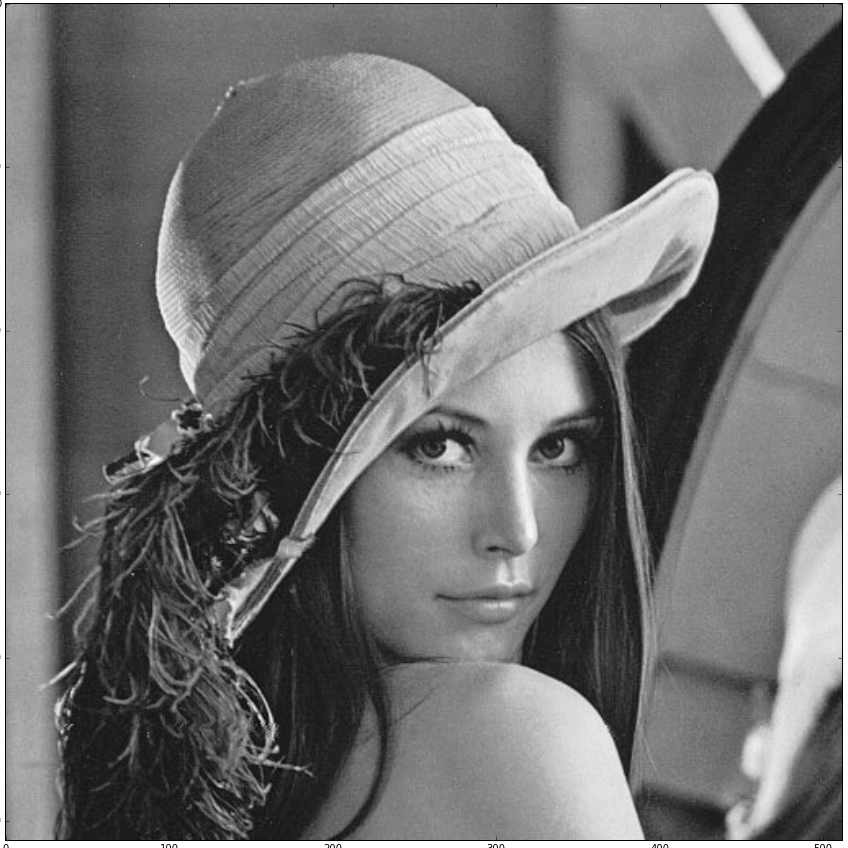
\includegraphics[width=\textwidth]{./Lena-gray}
    \caption{Original image}
    \label{pic-lena}
  \end{subfigure}
  \begin{subfigure}[t]{0.32\textwidth}
    \centering
    \captionsetup{justification=centering,margin=0.1cm}
    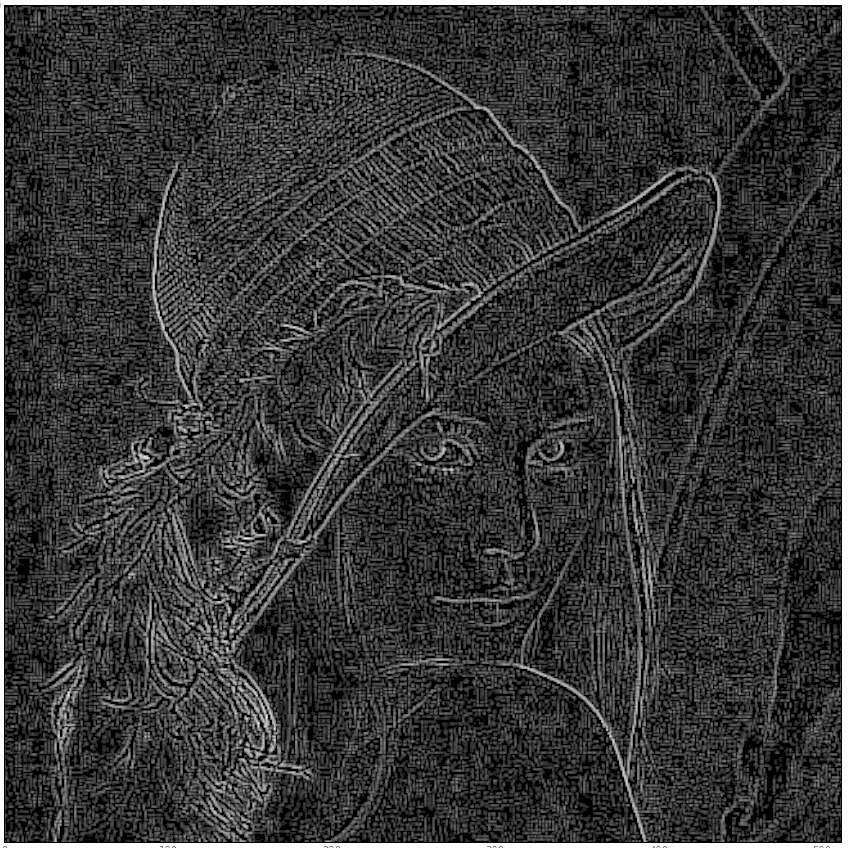
\includegraphics[width=\textwidth]{./Lena-midget_off}
    \caption{Layer 1}
    \label{pic-lena-M-OFF}
  \end{subfigure}
  \begin{subfigure}[t]{0.32\textwidth}
    \centering
    \captionsetup{justification=centering,margin=0.1cm}
    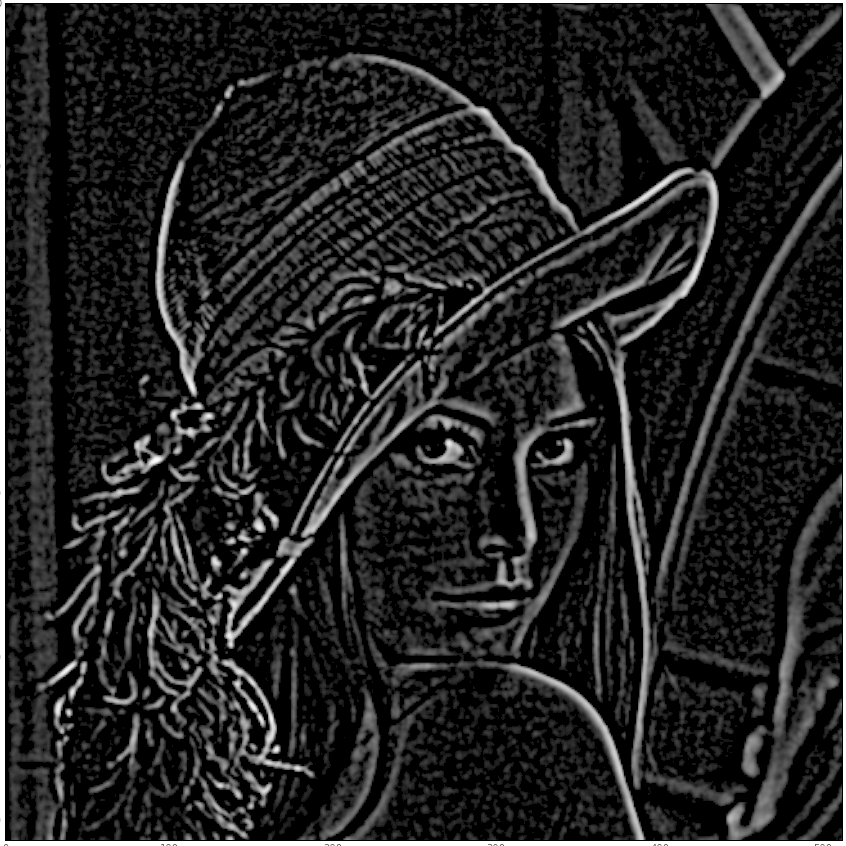
\includegraphics[width=\textwidth]{./Lena-midget_on}
    \caption{Layer 2}
    \label{pic-lena-M-ON}
  \end{subfigure}
  \begin{subfigure}[t]{0.32\textwidth}
    \vspace*{0.8em}
    \centering
    \captionsetup{justification=centering,margin=0.1cm}
    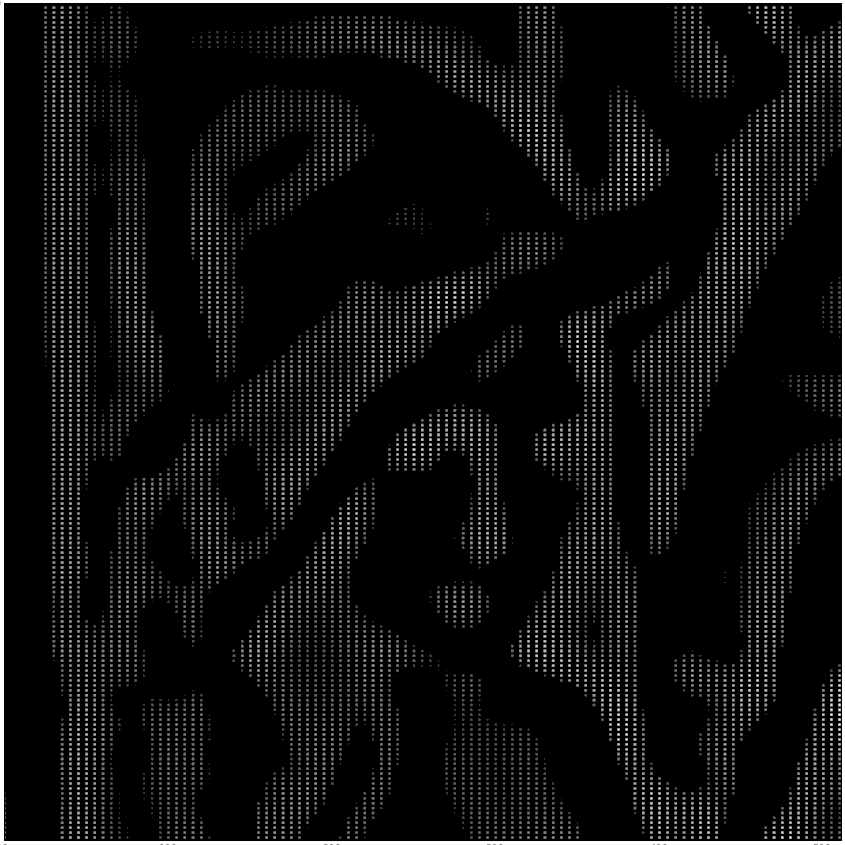
\includegraphics[width=\textwidth]{./Lena-parasol_off}
    \caption{Layer 3}
    \label{pic-lena-P-OFF}
  \end{subfigure}
  \begin{subfigure}[t]{0.32\textwidth}
    \vspace*{0.8em}
    \centering
    \captionsetup{justification=centering,margin=0.1cm}
    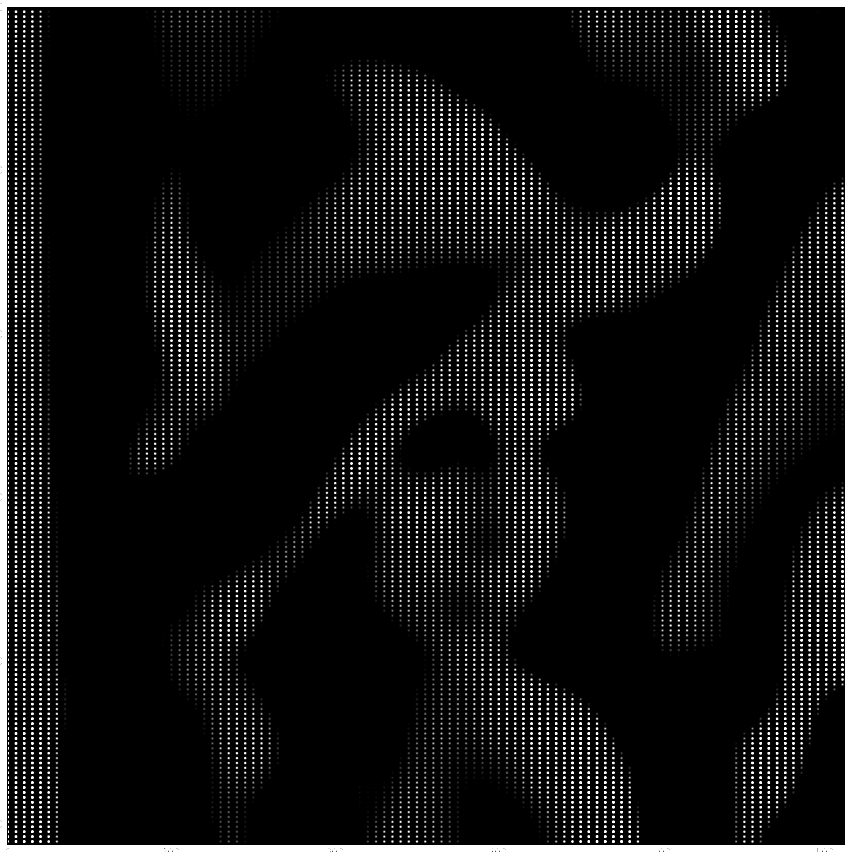
\includegraphics[width=\textwidth]{./Lena-parasol_on}
    \caption{Layer 4}
    \label{pic-lena-P-ON}
  \end{subfigure}
  \caption{Results of simulating ganglion cell layers (convolved images were enhanced for better contrast)}
  \label{fig-convolution-results}
\end{figure}

In order to check the validity of the generated spikes, a reconstruction procedure is employed (Equation \ref{eq:reconstruction}). Each coefficient in $C$ has an origin layer $w$, a value $c$ and a position ($k$, $l$). For all coefficients in $C$, a DoG from it's respective layer will be weighed by it's value and be added at the it's position to the reconstructed image $R$. The procedure is based on the assumption that the DoG are orthogonal basis. Figure \ref{pic-unfiltered-spikes} shows the result of the image reconstruction procedure without any redundancy correction applied.

\begin{equation}
  R(x,y) = \sum_{i}^{} \sum_{j}^{} \sum_{w}^{} C_{w}(i - x, j - y)DoG_{w}(i, j)
  \label{eq:reconstruction}
\end{equation}

\begin{figure}[hbt]
  \centering
  \begin{subfigure}[t]{0.3\textwidth}
    \centering
    \captionsetup{justification=centering,margin=0.1cm}
    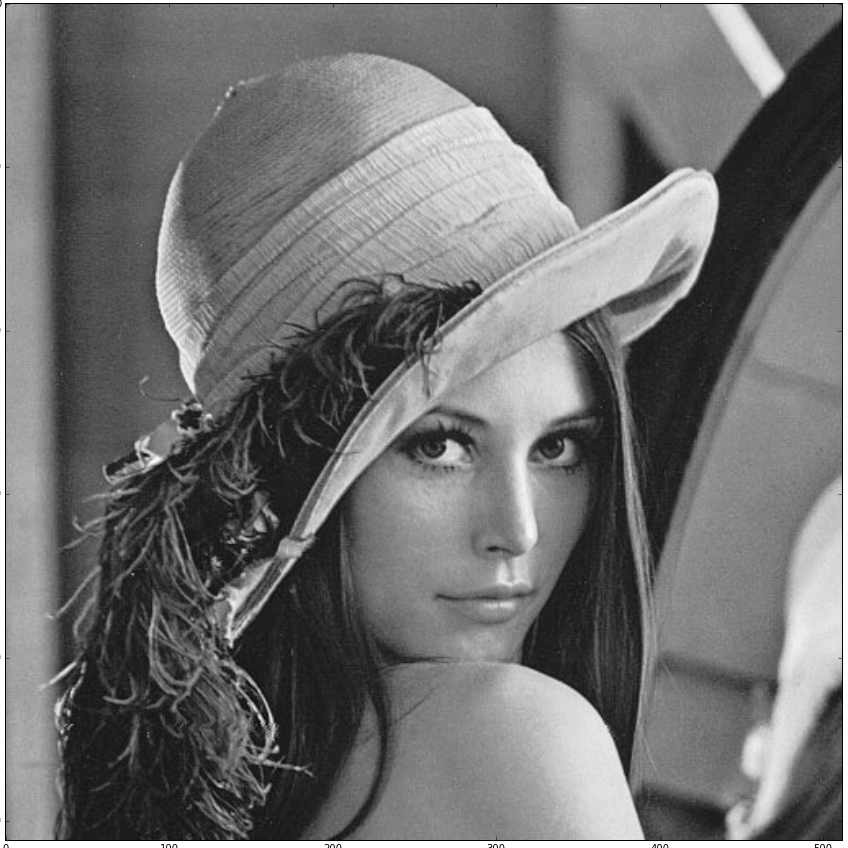
\includegraphics[width=\textwidth]{./Lena-gray}
    \caption{Original image}
  \end{subfigure}
  \begin{subfigure}[t]{0.3\textwidth}
    \centering
    \captionsetup{justification=centering,margin=0.1cm}
    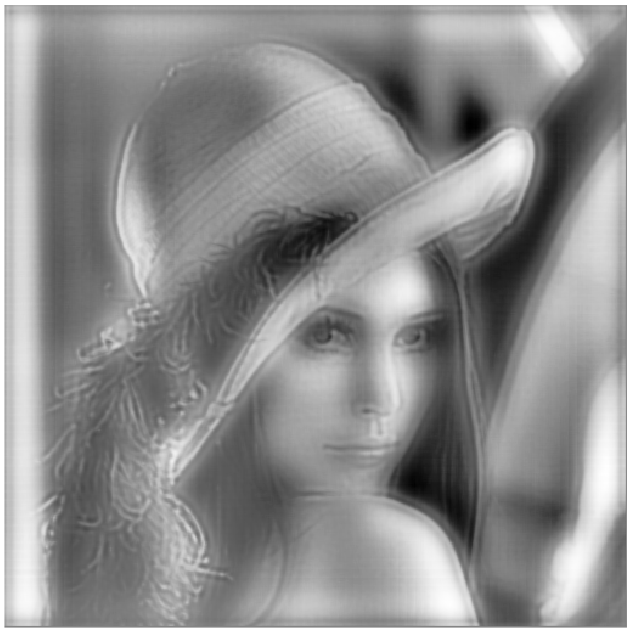
\includegraphics[width=\textwidth]{./final_results-unfiltered}
    \caption{100\% of raw spikes}
    \label{pic-unfiltered-spikes}
  \end{subfigure}
  \caption{Reconstruction results without overlap correction.}
\end{figure}

The eye is unlikely to provide unnecessary information to the brain, that is redundant information is filtered somehow before it's delivered. In the retina, lateral inhibition is the most likely candidate to minimize information redundancy. It's still a matter of discussion where and by which cells is lateral inhibition performed in the retina. It is most likely to happen in layers prior to the ganglion cell layer. The DoG kernels are only an approximately orthogonal basis, thus the resulting coefficients from the convolutions in Algorithm \ref{code-focal-conv} suffer from redundant information. That is, two neighbouring pixels might contain information that represent the same feature in the image. The main issue with this redundancy is that neighbouring coefficients might encode almost the same information with a similar value. Since the value provides the order of the spikes, this phenomenon will push other important coefficients into the later, less important, parts of the spike representation. In order to correct for redundancy, FoCal performs a second step (Algorithm \ref{code-focal-corr}).

\begin{algorithm}[htb]
  \caption{FoCal, Part 2}
  \label{code-focal-corr}
  \begin{algorithmic}
    \algrestore{bkbreak}
    \Procedure{Correction}{coeffs $C$, correlations $Q$}
    \State $N \leftarrow \emptyset$ \Comment{Corrected coefficients}
    \Repeat
    \State $m \leftarrow max(C)$
    \State $M \leftarrow M \cup m$
    \State $C \leftarrow C \setminus m$
    \ForAll{$ c \in C$} \Comment{Adjust all remaining c}
    \If{$Q(m, c) \neq 0$} \Comment{Adjust only near}
    \State $c \leftarrow c - m \times Q(m, c)$
    \EndIf
    \EndFor
    \Until{$C = \emptyset$}
    \State \textbf{return} $M$
    \EndProcedure
  \end{algorithmic}
\end{algorithm}

All the coefficients that where obtained from Algorithm \ref{code-focal-conv}, are put in a set $C$. For every step of the correction procedure the maximum coefficient is searched and its spatially surrounding pixels in all layers (Figure \ref{fig:focal2}) will be adjusted according to the correlation due to overlap between the maximum coefficient's convolution kernel and the other layer's kernels. The bold square in Figure \ref{fig:overlap} shows the overlap of two $3\times3$ kernels of neighbouring pixels, a similar overlap is considered for the interaction between layers.
\begin{figure}[htb]
  \centering
  \begin{subfigure}[t]{0.68\textwidth}
  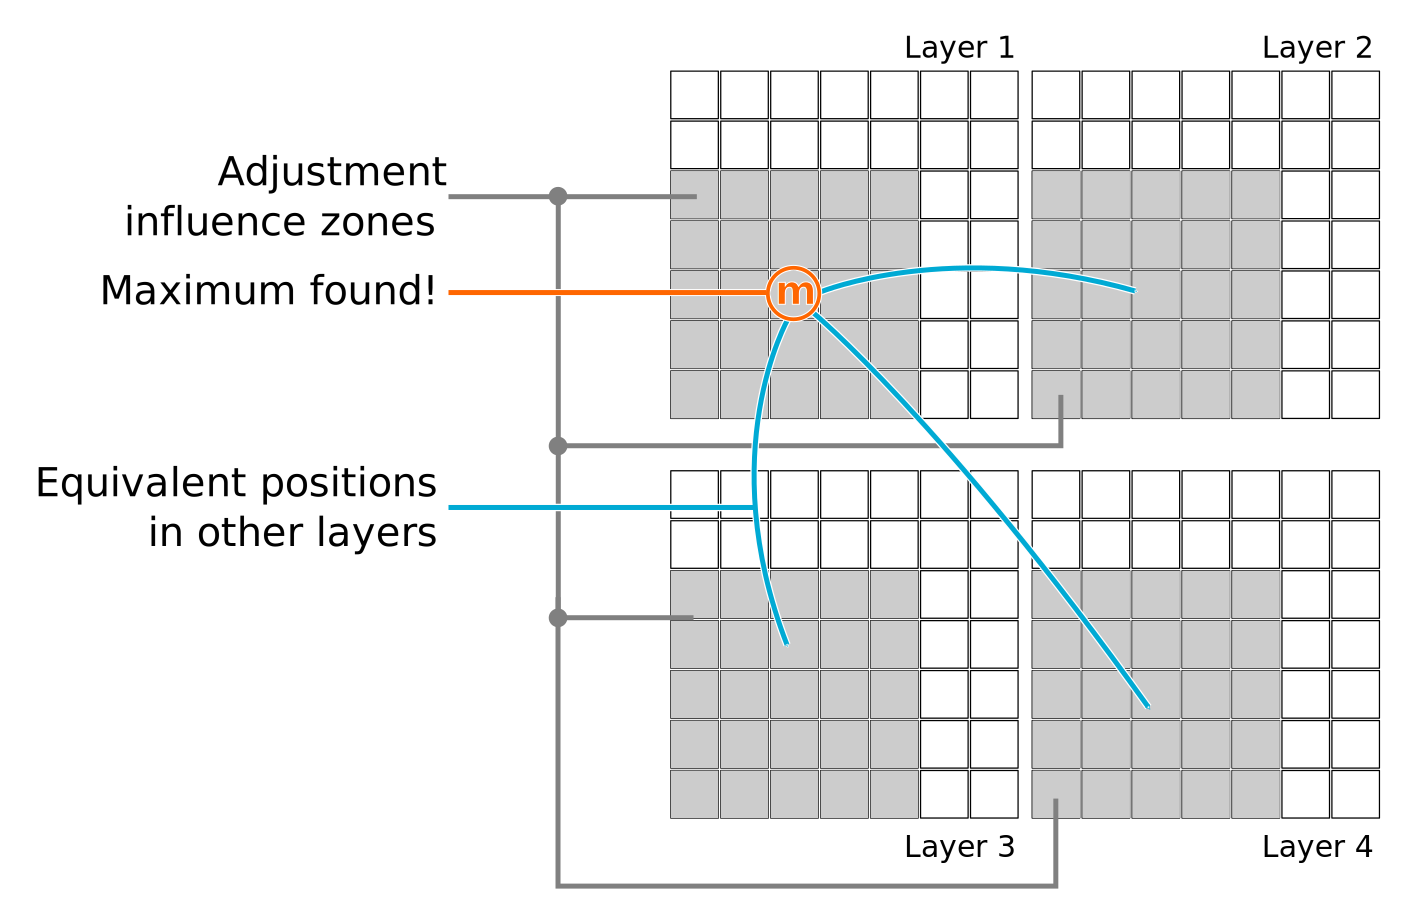
\includegraphics[width=\textwidth]{correction_adjustment}
  \caption{FoCal correction influence zones.}
  \label{fig:focal2}
  \end{subfigure}
  \hfill
  \begin{subfigure}[t]{0.29\textwidth}
  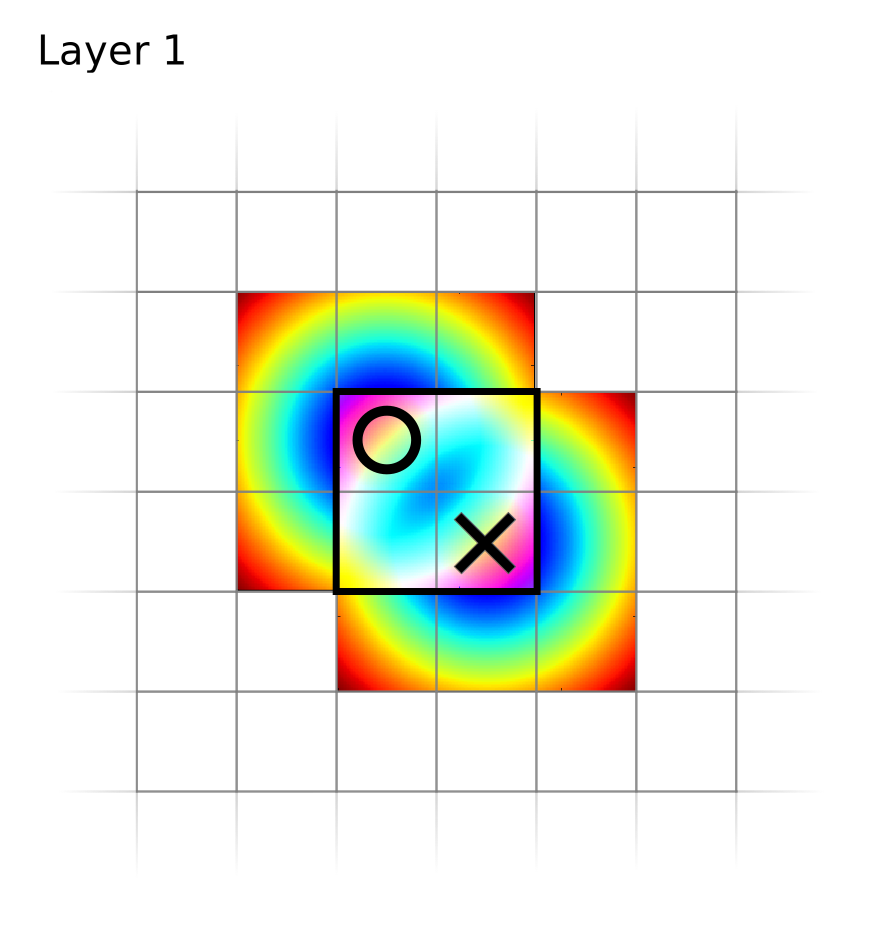
\includegraphics[width=\textwidth]{./coefficient_overlap}
  \caption{Kernel overlap}
  \label{fig:overlap}
  \end{subfigure}
\end{figure}

After this correction algorithm is applied only non-redundant spikes are preserved, this results in a much better reconstruction (Figure \ref{pic-100pc-spikes}). Not only is it more visually pleasing, but the fidelity of the reconstruction has been tested quantitatively; another interesting result is that only 10\% of the rank-ordered and FoCal corrected spikes are needed to preserve 90\% of the visually important information~\cite{basab-thesis}.

\begin{figure}[hbt]
  \centering
  \begin{subfigure}[t]{0.3\textwidth}
    \centering
    \captionsetup{justification=centering,margin=0.1cm}
    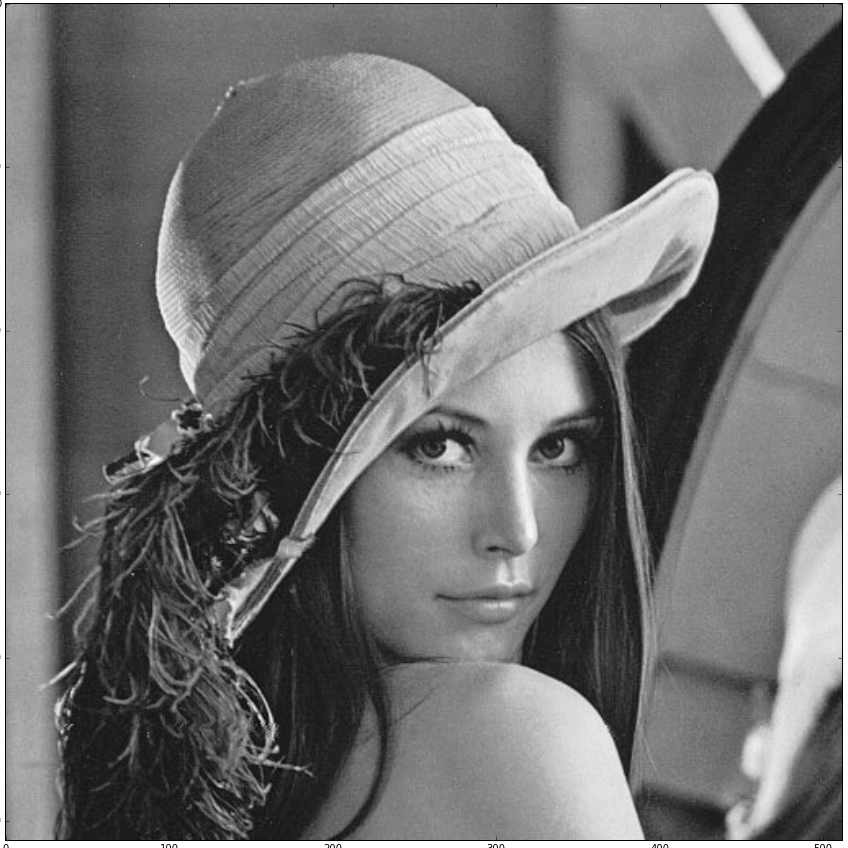
\includegraphics[width=\textwidth]{./Lena-gray}
    \caption{Original image}
    \label{pic-original-lena}
  \end{subfigure}
  \begin{subfigure}[t]{0.3\textwidth}
    \centering
    \captionsetup{justification=centering,margin=0.1cm}
    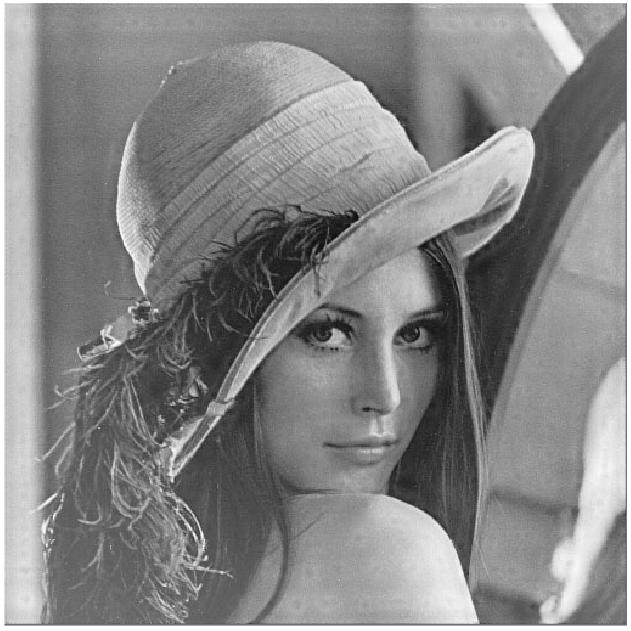
\includegraphics[width=\textwidth]{./final_results-focal-100}
    \caption{100\% of \emph{corrected} spikes}
    \label{pic-100pc-spikes}
  \end{subfigure}
  \begin{subfigure}[t]{0.3\textwidth}
    \centering
    \captionsetup{justification=centering,margin=0.1cm}
    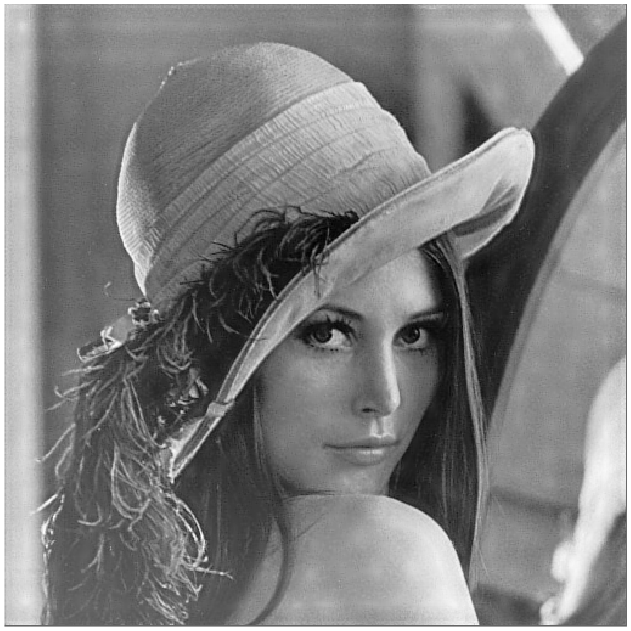
\includegraphics[width=\textwidth]{./final_results-focal-30pc}
    \caption{30\% of \emph{corrected} spikes}
    \label{pic-30pc-spikes}
  \end{subfigure}
  \caption{Results of reconstruction procedure}
  \label{fig-reconstruction}
  \vspace*{-10pt}
\end{figure}



\subsubsection{Implementation details}
Different ways of applying convolutions to images on a GPU where implemented and evaluated. The first one, the \textbf{naïve approach}, implies a discrete convolution with the full 2D kernels. Since we are using squared kernels, this means $N^2 \times W \times H$ operations for a $W\times H$ image using a kernel of width $N$. As expected, performance drops quickly and the biggest problem for this approach was that biggest kernel ($243\times243$ elements) requires more resources than the GPU's constant memory can provide (240 KBytes vs. 64 KBytes). This results in execution errors that may only be fixed using memory with greater latency to store the convolution kernel. 


The second approach to perform a 2D DoG convolution with an image is to rely on \textbf{kernel separability}. A convolution kernel $K$ is said to be \emph{separable} if $K = K_{1} \ast K_{2} \dots K_{n}$. Gaussian kernels are separable (Eq. \ref{eq:Gto1D}). and, fortunately a DoG is merely the subtraction of them (Eq. \ref{eq:DoG2G}).

\begin{equation}
O = I \ast DoG = I \ast G_{c} - I \ast G_{s}
\label{eq:DoG2G}
\end{equation}

Applying the algebraic properties of convolutions and the fact that Gaussian kernels are separable, the full 2D DoG convolution can be performed using four 1D separated ones (Eq. \ref{eq:DoGto1D}).

\begin{equation}
O = I \ast DoG = G_{v,c} \ast G_{h,c} \ast I - G_{v,s} \ast G_{h,s} \ast I 
\label{eq:DoGto1D}
\end{equation}

The main advantage of the separated kernel approach is a reduction of the number of operations needed ($4N\times W \times H$). An exception happens for the $3\times 3$ kernel, in this case there are 12 operations vs. the 9 needed for the naïve approach.


The last approach, \emph{Tiled Convolution} is reported by Advanced Micro Devices (AMD)~\cite{tiled-convolution}. They only present kernels of size $3\times3$, but we have an $11\times11$ convolution working; we are still developing solutions for the larger kernels. 



Convolution alone is a compute intensive task and we obtain about 12 frames-per-second (FPS) on videos with $640\times360$ 8-bit grayscale pixel resolution. Encoding was carried out using a desktop computer running 64-bit GNU/Linux, with a Core i5-4570 4-core CPU @ 3.20~GHz processor with 8~GBytes of 64-bit DDR3 RAM @ 1600~MHz and a GeForce GT 720 GPU with 192 CUDA cores @ 797~MHz, 1~GBytes of 64-bit DDR3 RAM @ 1800~MHz. %\\

\begin{table}[hbt]
  \begin{center}
    \caption{Convolution performance comparison.}
    \bgroup
    \def\arraystretch{1.4}
    \begin{tabular}{l c c c c}
      &
      \begin{minipage}{2cm}\centering Layer 0\vspace*{0.1cm}\end{minipage} & 
      \begin{minipage}{2cm}\centering
        Layer 1\vspace*{0.1cm}\end{minipage}& 
      \begin{minipage}{2cm}\centering
        Layer 2\vspace*{0.1cm}\end{minipage}& 
      \begin{minipage}{2cm}\centering
        Layer 3\vspace*{0.1cm}\end{minipage}\\
      \hline 
      
      Naïve     & 0.0009s & 0.0031s & 0.0587s & N/A$^{1,2}$ \\ 
      Separated & 0.0021s & 0.0055s & 0.0172s & 0.0472s \\ 
      % x, y, 0.01756, 0.04500
      Tiled     & 0.0009s & 0.0044s & 0.1643 & N/A$^2$\\
    \end{tabular} 
    \egroup
    {
      \footnotesize 
      \begin{center}
        $^1$ Unable to fit convolution kernel into constant memory.\\
        $^2$ Unable to compile OpenCL code.
      \end{center}
    }
  \end{center}
  \vspace*{-5pt}
\end{table}

The performance of convolution in GPUs is bound by memory transfers, even if some of the information is reused.



In the retina, redundancy of information is reduced via lateral inhibition 
prior to any ganglion cell activity. In this algorithm, we perform a correction 
on the convolved images by adjusting the pixel values
according to the correlation between convolution kernels 
(Alg.~\ref{code-focal-corr}). The results of using correction 
(Fig.~\ref{pic-unfiltered-spikes}) or not (Fig.~\ref{pic-100pc-spikes}) show 
that the convolution stage can only provide redundant information. Furthermore, 
using only 30\% of the corrected weights still provides enough visual 
information to reconstruct the original image~\cite{basab-model}.

Correcting the spikes for redundancy is a highly time consuming task which
might be better suited for event-based programming, such as the one found on 
the SpiNNaker platform. We are still working on an implementation for this 
approach.\\




12fps is for good most phenomenon, full image encoding

This probably happens only once every so many ms


\subsection{A dynamic vision sensor emulator}

Output what a DVS does but with a camera as a source

Convolution of current and past frames ? centre - current / surround - past

Per-pixel adaptive threshold keeps fast changing pixels from spiking constantly, emulates refractory period of cells.



A second way of encoding is to simulate the early stages of the retina, which 
sense changes in intensity on the photoreceptors. This is quite similar to what 
real Dynamic Vision Sensors (DVS) do but with limited dynamic range and lower 
temporal resolution~\cite{aer-retina-bernabe,dvs-zurich}. The main advantage is 
that no specialized hardware is needed and the operation is so fast that any 
recent computer should be able to do it. For this type of encoding procedure we 
hypothesize that the bigger the change, the sooner a cell would spike and, 
thus, we can obtain a spike timings given the difference of two video frames. 
So far we can process about 20 and 25 FPS using a Numpy and an OpenCL back-end, 
respectively (using the same hardware set-up previously described). Although 
it's currently a good approximation, more research on this algorithm is needed 
to better approximate to biology. 

